%Chapter 2

\renewcommand{\thechapter}{2}
\thispagestyle{empty}
\chapter{Image Texture Analysis}

\section{Texture Analysis Using GLCM Algorithm}

\subsection{Overview}
Grey-Level Co-occurrence Matrix (GLCM) is a common method to represent the distance and angular spatial relationship of the image with a whole segment or sub-segment of specific size. It is created from the array of pixels of an image. Texture is a term to describe an image in another way. The texture measurements of GLCM was firstly proposed by Haralick in the 1970s for image classification\cite{Haralick}. Since then it has been widely applied in many fields to solve some specific problems such as the classification of breast lesions on ultrasound (BUS) images\cite{Gomez} and the analysis of synthetic aperture radar (SAR) imagery\cite{Umasankar}. In general, GLCM is a statisitical method for calculating the frequency between the pixel of reference and its neighbor. It is created by counting the total number of pairs occurring in the array of pixels. Each pair consists of the reference pixel value and its corresponding neighbor pixel value. Given the symbol $G_{(i,j)}$ which represents the element in GLCM,  we have the parameter i that means the reference pixel value and j that means the corresponding neighbor pixel value of the parameter i. In creating GLCM, there are two major parameters that need to be considered, angle direction and offset. The angle direction of GLCM specifies the possible location of the neighbor pixel in regard to its reference pixel. Generally speaking, there are four basic GLCM directions that are the $0^0$ $P_0$, the $90^0$ $P_{90}$ and the diagonal degree that includes the $45^0$ representing bottom left to to top right $P_{45}$ and the $135^0$ representing top left to bottom right $P_{135}$ shown in Figure 2.1. 
\begin{figure}[!t]
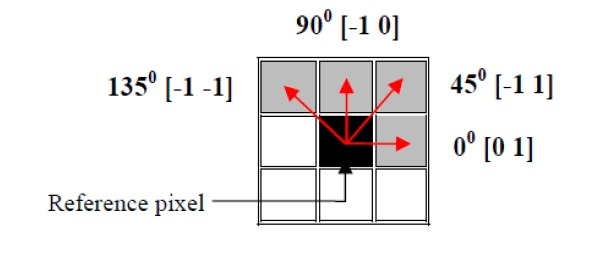
\includegraphics{GLCM_direction_sample}
\caption{GLCM angle directions for calculating textural features\cite{Biswajit}}
\end{figure}
In addition, by considering the symmetric property, the value of each element is doubled. In general, there is a fifth GLCM created by considering the average of GLCM along with four angle directions. Offset means the distance between the reference pixel value and its neighbor. Given $E_{(i,j)}$ which is the element in the array of pixels representing an image, if we consider $E_{(i,j)}$ as reference, the $E_{(i,j+n)}$ where n means the value of the offset is the neighbor in horizontally, to the right. Similarly, the the $E_{(i-n,j+n)}$ is the diagonal neighbor  from bottom left to top right, the $E_{(i-n,j)}$ is the vertical neighbor from bottom to top, and the $E_{(i-n,j-n)}$ is diagonal neighbor from bottom right to top left.\par
For example, given a 3-by-6 array  
\begin{align*}
I = 
\begin{bmatrix}
& 1 & 1 & 5 & 6 & 8 & 8 &\\
& 2 & 3 & 5 & 7 & 0 & 2 &\\
& 0 & 2 & 3 & 5 & 6 & 7 &
\end{bmatrix}
\end{align*}
The figure represents a sub-region of an image with pictorial information. GLCM is an m-by-m matrix where m is the gray levels of an image. For image I, since the pixel value ranges from 0 to 8, the gray level is 9. Thus, a 9-by-9 matrix is created as a part of the whole GLCM in $0^0$ angle direction with offset 1. Under this circumstance, considering $E_{(1, 1)} = 1$ as the reference pixel value, its neighbor is $E_{(1, 2)} = 1$. Thus, the $G_{(1,1)}$ is currently equal to 1. In the meantime, we can find that the $G_{(0, 2)} = 2$, because when we treat the pixel value 0 as the reference, the pixel value 2 as the corresponding neighbor appears twice in $E_{(2,6)}$ and $E_{(3,2)}$.    
\begin{table}[!h]
\begin{center}
\renewcommand{\arraystretch}{0.5}
\begin{tabular}{c | c c c c c c c c c|}
 \backslashbox{\textit{reference}}{\textit{neighbor}} & 0 & 1 & 2 & 3 & 4 & 5 & 6 & 7 & 8 \\
\hline
 0 & 0 & 0 & 2 & 0 & 0 & 0 & 0 & 0 & 0 \\
 1 & 0 & 1 & 0 & 0 & 0 & 0 & 0 & 0 & 0 \\
 2 & 0 & 0 & 0 & 2 & 0 & 0 & 0 & 0 & 0 \\
 3 & 0 & 0 & 0 & 0 & 0 & 2 & 0 & 0 & 0 \\
 4 & 0 & 0 & 0 & 0 & 0 & 0 & 0 & 0 & 0 \\
 5 & 0 & 0 & 0 & 0 & 0 & 0 & 2 & 1 & 0 \\
 6 & 0 & 0 & 0 & 0 & 0 & 0 & 0 & 1 & 1 \\
 7 & 1 & 0 & 0 & 0 & 0 & 0 & 0 & 0 & 0 \\
 8 & 0 & 0 & 0 & 0 & 0 & 0 & 0 & 0 & 1 \\
\end{tabular}
\caption{The sub-region of GLCM in 0 degrees (offset = 1)}
\end{center}
\end{table}
By counting all reference pixel values, we achieve the GLCM shown in Table 2.1. Similarly, we create the different GLCM in the remaining three directions shown in Table 2.2, Table 2.3 and Table 2.4.
\begin{table}[!h]
\begin{center}
\renewcommand{\arraystretch}{0.5}
\begin{tabular}{c | c c c c c c c c c|}
 \backslashbox{\textit{reference}}{\textit{neighbor}} & 0 & 1 & 2 & 3 & 4 & 5 & 6 & 7 & 8 \\
\hline
 0 & 0 & 0 & 0 & 1 & 0 & 0 & 0 & 0 & 1 \\
 1 & 0 & 0 & 0 & 0 & 0 & 0 & 0 & 0 & 0 \\
 2 & 0 & 1 & 0 & 0 & 0 & 1 & 0 & 0 & 0 \\
 3 & 0 & 0 & 0 & 0 & 0 & 1 & 0 & 1 & 0 \\
 4 & 0 & 0 & 0 & 0 & 0 & 0 & 0 & 0 & 0 \\
 5 & 1 & 0 & 0 & 0 & 0 & 0 & 1 & 0 & 0 \\
 6 & 0 & 0 & 1 & 0 & 0 & 0 & 0 & 0 & 0 \\
 7 & 0 & 0 & 0 & 0 & 0 & 0 & 0 & 0 & 1 \\
 8 & 0 & 0 & 0 & 0 & 0 & 0 & 0 & 0 & 0 \\
\end{tabular}
\caption{The sub-region of GLCM in 45 degrees (offset = 1)}
\end{center}
\begin{center}
\renewcommand{\arraystretch}{0.5}
\begin{tabular}{c | c c c c c c c c c|}
 \backslashbox{\textit{reference}}{\textit{neighbor}} & 0 & 1 & 2 & 3 & 4 & 5 & 6 & 7 & 8 \\
\hline
 0 & 0 & 0 & 1 & 0 & 0 & 0 & 0 & 0 & 1 \\
 1 & 0 & 0 & 0 & 0 & 0 & 0 & 0 & 0 & 0 \\
 2 & 0 & 1 & 0 & 1 & 0 & 0 & 0 & 0 & 1 \\
 3 & 0 & 1 & 0 & 0 & 0 & 1 & 0 & 0 & 0 \\
 4 & 0 & 0 & 0 & 0 & 0 & 0 & 0 & 0 & 0 \\
 5 & 0 & 0 & 0 & 0 & 0 & 1 & 0 & 1 & 0 \\
 6 & 1 & 0 & 0 & 0 & 0 & 0 & 0 & 0 & 0 \\
 7 & 0 & 0 & 1 & 0 & 0 & 0 & 1 & 0 & 0 \\
 8 & 0 & 0 & 0 & 0 & 0 & 0 & 0 & 0 & 0 \\
\end{tabular}
\caption{The sub-region of GLCM in 90 degrees (offset = 1)}
\end{center}
\end{table}
\begin{table}
\begin{center}
\renewcommand{\arraystretch}{0.5}
\begin{tabular}{c | c c c c c c c c c|}
  \backslashbox{\textit{reference}}{\textit{neighbor}} & 0 & 1 & 2 & 3 & 4 & 5 & 6 & 7 & 8 \\
\hline
 0 & 0 & 0 & 0 & 0 & 0 & 0 & 1 & 0 & 0 \\
 1 & 0 & 0 & 0 & 0 & 0 & 0 & 0 & 0 & 0 \\
 2 & 0 & 0 & 1 & 0 & 0 & 0 & 0 & 0 & 1 \\
 3 & 0 & 1 & 0 & 1 & 0 & 0 & 0 & 0 & 0 \\
 4 & 0 & 0 & 0 & 0 & 0 & 0 & 0 & 0 & 0 \\
 5 & 0 & 1 & 0 & 0 & 0 & 1 & 0 & 0 & 0 \\
 6 & 0 & 0 & 0 & 0 & 0 & 0 & 0 & 1 & 0 \\
 7 & 1 & 0 & 0 & 0 & 0 & 1 & 0 & 0 & 0 \\
 8 & 0 & 0 & 0 & 0 & 0 & 0 & 0 & 0 & 0 \\
\end{tabular}
\caption{The sub-region of GLCM in 135 degrees (offset = 1)}
\end{center}
\end{table} 
Finally, through adding these four GLCM together and dividing it by 4, we have the fifth GLCM.

\subsection{Texture Measurements of GLCM}
The texture measurements of GLCM are calculated from the normalized GLCM. To achieve the normalized GLCM, each value in GLCM is divided by its total number of occurrences in the GLCM. Normally, the total number of occurrences is the number of valid reference pixels. For instance, if we create the GLCM from image I along with the $0^0$ direction with offset 1, the total number of occurrences is 15 because the reference pixels in the last column have no neighbors. Some basic functions will be used in calculating the texture features of GLCM\cite{Haralick}. Assuming that the parameter G represents the number of gray levels, the basic functions are defined as follows:\\
The probability of i as the reference pixel value in a gray-scale image:
\begin{equation}
    p_x(i) = \sum_{j=0}^{G-1}p(i,j) 
\end{equation}
The probability of j as the neighbor pixel value in a gray-scale image:
\begin{equation}
    p_y(j) = \sum_{i=0}^{G-1}p(i,j)
\end{equation}
The probability of k which is the summary of the reference and neighbor pixel value:
\begin{equation}
    p_{x+y}(k) = \sum_{i=0}^{G-1}\sum_{j=0}^{G-1} p(i,j) \; where\; k = i + j\;(k=0,1,\ldots,2G-2)
\end{equation}
The probability of k which is the difference between reference and neighbor pixel value:
\begin{equation}
    p_{x-y}(k) = \sum_{i=0}^{G-1}\sum_{j=0}^{G-1} p(i,j) \; where\; k = |i - j|\;(k=0,1,\ldots,G-1)
\end{equation}
The mean value of $p_x$:
\begin{equation}
\mu_x = \sum_{i=0}^{G-1}ip_x(i)=\sum_{i=0}^{G-1}\sum_{j=0}^{G-1} ip(i,j)
\end{equation}
The standard deviation of $p_x$:
\begin{equation}
\sigma_x = \sqrt{\sum_{i=0}^{G-1}(i-\mu_x)^2p_x(i)}
\end{equation}
The mean value of $p_y$:
\begin{equation}
\mu_y = \sum_{j=0}^{G-1}jp_j(j)=\sum_{i=0}^{G-1}\sum_{j=0}^{G-1} jp(i,j)
\end{equation}
The standard deviation of $p_y$:
\begin{equation}
\sigma_y = \sqrt{\sum_{j=0}^{G-1}(j-\mu_y)^2p_y(j)}
\end{equation}
Consequently, due to the normalized GLCM and the basic functions listed above, the texture feature parameters of GLCM are defined as follows\cite{Haralick}:\\
1. Energy, Homogeneity, Angular Second Moment(ASM): 
\begin{equation}
ASM = \sum_{i=0}^{G-1}\sum_{j=0}^{G-1}\{p(i,j)\}^2
\end{equation}
The feature ASM is used to measure the homogeneity of an image\cite{Peng}. The value of ASM is usually more than $G^{-2}$ but less than 1. If a GLCM only has a few relatively high value of $p(i,j)$, the homogeneous scene contains only a few gray levels\cite{Albregtsen}.\\
2. Inertia, Contrast(CON):
\begin{equation}
CON = \sum_{k=0}^{G-1}k^2p_{x-y}(k)
\end{equation}
The feature CON is used to measure the local difference within an image. Its value depends on the position of pixels. In general, the more elements away from the diagonal, the higher value the feature has. Otherwise, the more elements in the diagonal, the lower value it has.\\ 
3. Correlation(COR):
\begin{equation}
COR = \frac{\sum_{i=0}^{G-1}\sum_{j=0}^{G-1}(i-\mu_x)(j-\mu_y)p(i,j)}{\sigma_x\sigma_y} = \frac{\sum_{i=0}^{G-1}\sum_{j=0}^{G-1}(ij)p(i,j)-\mu_x\mu_y}{\sigma_x\sigma_y}
\end{equation}
The feature COR is used to measure the linear dependence of gray levels between the specific position of pixels relative to each other. It depends on how an image is organized. The value of COR is more than -1 but less than 1.\\
4. Sum of Squares, Variance(VAR):
\begin{equation}
VAR = \sum_{i=0}^{G-1}\sum_{j=0}^{G-1}(i-\mu_x)^2p(i,j) \\
    = \sum_{i=0}^{G-1}(i-\mu_x)^2p_x(i)
\end{equation}
The feature VAR measures the degree of how the elements differ from the average value of $p(i,j)$. \\
5. Local Homogeneity, Inverse Difference Moment(IDM):
\begin{equation}
IDM = \sum_{i=0}^{G-1}\sum_{j=0}^{G-1}\frac{1}{1+(i-j^2)}p(i,j)
\end{equation}
The feature IDM is affected by the homogeneity of an image, because of the weighting factor $1+(i - j)^2$. Thus, the value is high if the image is homogeneous, while the value is low if the image is inhomogeneous.\\
6. Sum Average(SAV):
\begin{equation}
SAV = \sum_{k=0}^{2G-2}kp_{x+y}(k)
\end{equation}
7. Sum Entropy(SEN):
\begin{equation}
SEN = -\sum_{k=0}^{2G-2}p_{x+y}(k)\log(p_{x+y}(k))
\end{equation}
8. Sum Variance(SVA):
\begin{equation}
SVA = \sum_{k=0}^{2G-2}(k-SEN)^2p_{x+y}(k)
\end{equation}
9. Entropy(ENT):
\begin{equation}
ENT = - \sum_{i=0}^{G-1}\sum_{j=0}^{G-1}p(i,j)\log(p(i,j))
\end{equation}
10. Difference Entropy(DEN):
\begin{equation}
DEN = -\sum_{k=0}^{G-1}p_{x-y}(k)\log(p_{x-y}(k))
\end{equation}
11. Difference Variance(DVA):
\begin{equation}
DVA = \sum_{k=0}^{G-1}k^2p_{x-y}(k)
\end{equation}
12. Dissimilarity(DIS):
\begin{equation}
DIS = \sum_{i=0}^{G-1}\sum_{j=0}^{G-1}|i-j|p(i,j)
\end{equation}
13. Cluster shade(CLS):
\begin{equation}
CLS = \sum_{i=0}^{G-1}\sum_{j=0}^{G-1}(i+j-\mu_x-\mu_y)^3p(i,j) = \sum_{i=0}^{G-1}\sum_{j=0}^{G-1}(i+j-2\mu_x)^3p(i,j)
\end{equation}
14. Cluster prominence(CLP):
\begin{equation}
CLP=\sum_{i=0}^{G-1}\sum_{j=0}^{G-1}(i+j-\mu_x-\mu_y)^4p(i,j) = \sum_{i=0}^{G-1}\sum_{j=0}^{G-1}(i+j-2\mu_x)^4p(i,j)
\end{equation}
15. Minimum probability(MIP):
\begin{equation}
MIP = \min(p(i,j))
\end{equation}
16. Maximum probability(MAP):
\begin{equation}
MAP=max(p(i,j))
\end{equation}
17. Mean(MEA):
\begin{equation}
MEA = \sum_{i=0}^{G-1}i\sum_{j=0}^{G-1}p(i,j) = \mu_x
\end{equation}
18. Relative minimum pixel intensity(IMIN):
\begin{equation}
IMIN = \frac{min(J(x,y))}{mean(J(x,y))}
\end{equation}
19. Relative maximum pixel intensity(IMAX):
\begin{equation}
IMAX = \frac{max(J(x,y))}{mean(J(x,y))}
\end{equation}
20. Mean value of pixel intensity(IMEA):
\begin{equation}
IMEA = mean(J(x,y))
\end{equation}
The J(x,y) represents the 12-bit diffraction image before normalization. Based on Haralick's research\cite{Thati}, the texture features defined above are categorized into three groups named as \textit{Contrast}, \textit{Uniformity} or \textit{Orderliness} of pixels, and \textit{Correlation} and \textit{statistic} over the pixels. In Group 1, the measures of Contrast include CON, DIS, IDM, VAR, SVA and DVA. In Group 2, the measures of Uniformity or Orderliness of pixels consist of MAP, ASM, ENT, DEN, SEN, CLS and CLP. In group 3, the measures of Correlation and other descriptive statistics contain COR, MIP, MEA, IMIN, IMAX, IMEA and SAV.\par
These feature parameters facilitate representing an image from the textural level. For example, given two different types of diffraction images taken both from camera with an s-polarizer and p-polarizer in front as the Figure 2.2 shows, we examine three basic feature parameters from different groups. The feature CON in group 1 describes the difference moment of image pixel matrix by measuring the amount of local variations present in an image. As for the images shown in Figure 2.2, the CON value of the cell image is 2.511395, while the value of the debris image is 104.8141, which is calculated using equation 2.10. The Debris image has the larger CON value than the Cell image because the Cell image has a lower amount of local variations than the Debris image as the Figure 2.2 shows. The feature ASM in group 2 describes the degree of homogeneity that an image has by measuring the total number of dominant gray-tone transitions. Through calculation, the value of the cell image is 0.031834, whereas the value of the debris image is 0.000838. Due to the fact that the cell image has many fewer dominant gray-tone transitions than the Debris image, the ASM of Cell image is higher than the Debris image. Another feature COR in group 3 describes the gray-tone linear-dependencies by considering the amount of linear structure across the image. The debris image has a lower value than the cell image because the Debris image contains a noise sample which is usually uncorrelated. Meanwhile, by comparing the COR value of the Debris image along different directions, we find that the values along $0^0$ and $90^0$ are higher than the values along $45^0$ and $135^0$ because the Debris image has a certain amount of linear structure along these two lines. 
\begin{figure}[!t]
\centering
  \begin{subfigure}[b]{0.4\textwidth}
    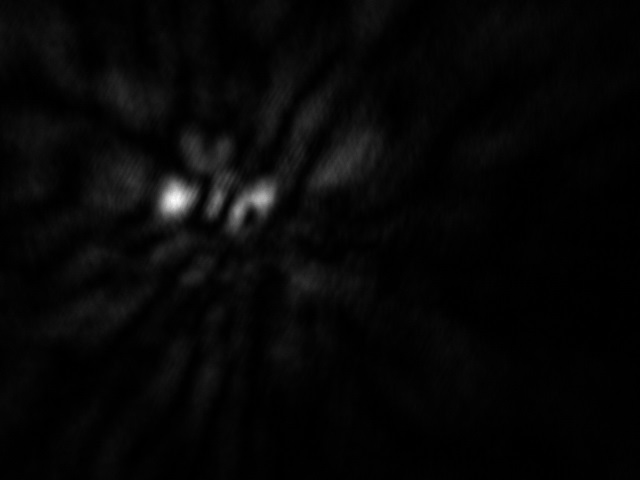
\includegraphics[width=\textwidth]{diffraction_image/2015040117594700116-2}
    \caption{Cell image}
  \end{subfigure}
  \begin{subfigure}[b]{0.4\textwidth}
    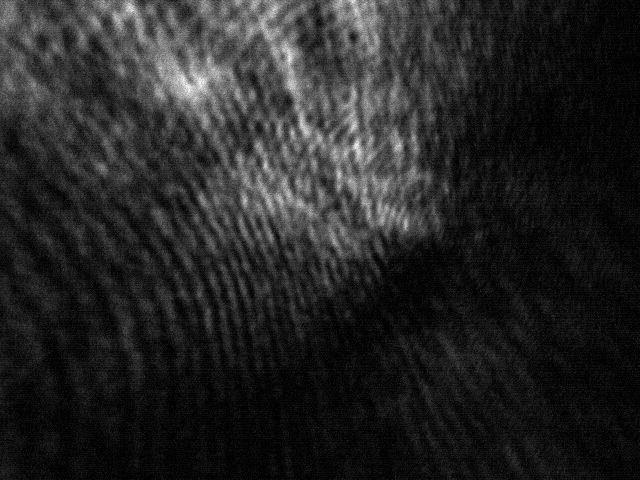
\includegraphics[width=\textwidth]{diffraction_image/2015040117594700009-2}
    \caption{Debris image}
  \end{subfigure}
  \caption{Two diffraction images with different types captured with s-polarizer}
\end{figure}
\section{Development of GLCM Feature Calculation Application}
\subsection{Problem Statement}
Since the GLCM as a texture analysis approach is so popular, some tools provide the built-in method to create the GLCM, such as MATLAB. However, for users who do not have the experience on MATLAB, it is hard to utilize the built-in method there. If users have little knowledge or experience of MATLAB, it is inconvenient to implement a script for extracting GLCM texture feature parameters. Thus, an application for this purpose is needed. The application shall allow users to specify the image folder so that the application can automatically process all images in that folder. The application also shall allow users to customize the offset value and the direction for creating the GLCM. To expand the function, the application should enable users to have choices feature parameters in a single direction, a combination of directions, and all processed directions. Finally, the application shall automatically combine an image pair as a feature parameter example.  
\subsection{Class Diagram and GLCM Application Implementation}
\begin{figure}[!h]
\begin{center}
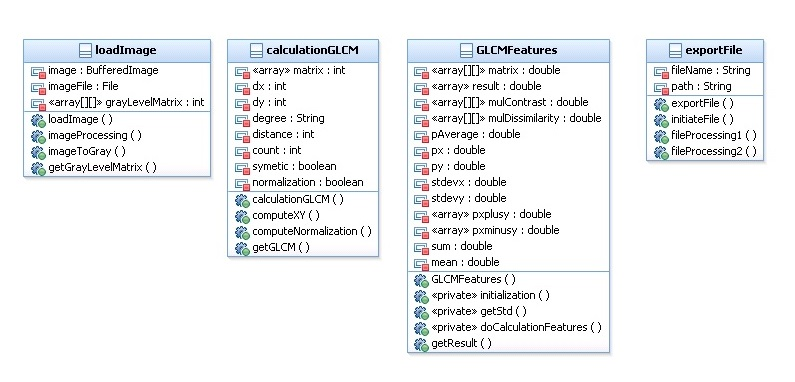
\includegraphics[width=4.25in]{class_diagram}
\end{center}
\renewcommand{\baselinestretch}{1}
\small\normalsize
\begin{quote}
\caption{The major classes for GLCM feature calculation application}
\label{fig2.2}
\end{quote}
\end{figure}
\renewcommand{\baselinestretch}{2}
\small\normalsize
Based on the problem statement above, the application should comprise several components which are loading images, converting into two-dimensional (2D) matrix, computing GLCM based on the 2D matrix, calculating features from GLCM, and exporting a comma-separated values (CSV) file that is used to store the desired result. Therefore, the major classes shown in Figure 2.3 are constructed to represent the attributes and operations within the application. To process the massive amount of images, the application loops the procedure consisting of class loadImage, class calculationGLCM, and class GLCMFeatures until no image remains. During each loop, all calculated features are stored using the ArrayList method. Finally, class exportFile extracts all features from the ArrayList and conducts them into a CSV file.\par
In this application, class loadImage is implemented by applying the Application Program Interface (API) Image I/O in JAVA library. The API provides a way of loading the image into its BufferedImage formats. It supports built-in methods for GIF, PNG, JPEG, BMP, and WBMP which are some different formats of image data. In JAVA, the BufferedImage which is a subclass of class Image describes an image with an accessible buffer of image data. The BufferedImage class, it is constructed by the raster of image data that represents a rectangular array of pixels. Thus, through applying these APIs, the image data is processed and generates a rectangular array of pixels whose size corresponds to the resolution of the image. for example, if the resolution of an image is 640x480, the raster of the image data is a 640-by-480 array of pixels. In the meantime, the range of image pixel depends on its color depth. For instance, the highest pixel value of an 8-bit image data is 256. \par
The calculationGLCM class takes the array of pixels that is the output of loadImage class as input and creates the specific GLCM due to other input parameters such as distance and angle. The mechanism for this class is going through all elements in the array of pixels, and for each element, finding its corresponding neighbor element with specific conditions. Meanwhile, if an element has no neighbor, it contributes nothing to GLCM. As a result, given an m-by-n array of pixels
\begin{align*}
I = 
\begin{bmatrix}
E(0,0) & E(0,1) & \ldots & E(0,n-1) \\
\vdots &         &         & \vdots \\
E(d,0) & E(d,1) & \ldots & E(d,n-1) \\
\vdots &         &         & \vdots \\
E(m-1,0) & E(m-1,1) & \ldots & E(m-1,n-1) 
\end{bmatrix}
\end{align*} where d is the offset value and considering the exception problem in programming,
to calculate GLCM along 0 degrees direction, a two dimension loop that counting the frequency starts from the element $E(0,0)$ and ends at the element $E(m-1, n-d)$; to calculate GLCM along 45 degrees direction, the loop starts from the element $E(d,0)$ and ends at the element $E(m-1, n-d)$; to calculate GLCM along 90 degrees direction, the loop starts from the element $E(d,0)$ and ends at the element $E(m-1, n-1)$; to calculate GLCM along 135 degrees direction, the loop starts from the element $E(d,d)$ and ends at the element $E(m-1, n-1)$. 
By applying class GLCMFeatures, all texture features are calculated from the GLCM created through class calculationGLCM. In this class, the method initialization() is implemented to calculate parameters $p_x(i)$, $p_y(j)$, $p_{x+y}(k)$, $p_{x-y}(k)$, $\mu_x$, $\mu_y$, $\sigma_x$ and $\sigma_y$ due to the equations from 2.1 to 2.8. Then, we implement the doCalculationFeatures() method that is responsible for calculating the 17 texture features of an image which are listed from equation 2.9 to 2.25.\par
Finally, the class exportFile is implemented for creating the result report in CSV format. Generally speaking, the common strategy is building a string with the comma. In this case, we utilize the StringBuilder method to construct the string in that format and apply the printWriter function to add it to a specific CSV file. 

\subsection{GLCM Application Verification}
Software verification as a part of software testing is an important procedure to ensure that the software implements all requirements. The two primary goals for software testing is finding bugs or defects and gaining confidence in the software\cite{Jiantao}. Traditionally, the testing methods are divided into white-box testing that tester examines the internal structure or workings of a program and black-box testing that tester examines the functionality without knowing the internal implementation and seeing the source code. To do the black-box testing, a test oracle which is a mechanism in software testing to determine whether a test has passed or not\cite{Kaner} is required. in the meanwhile, the test case which includes a set of test data as inputs, the expected outputs, and the execution condition is the central factor that is involved in the use of an oracle. As for the GLCM application, the input is an image and the output is the corresponding texture features based on the image's GLCM for system testing which is a high-level software testing process.\par
In this thesis research, there are MATLAB scripts implemented for research in selecting features to analyze the diffraction image\cite{Thati} and the C++ tool implemented for calculating texture features from GLCM. To verify them, we considered the black-box testing because the tester lacks sufficient knowledge in MATLAB and C++ programming language. However, by using the four diffraction images shown in Figure 2.4 as inputs for the testing process, these two tools produced different calculations for the texture features. 
\begin{figure}[!b]
  \begin{subfigure}[b]{0.5\textwidth}
    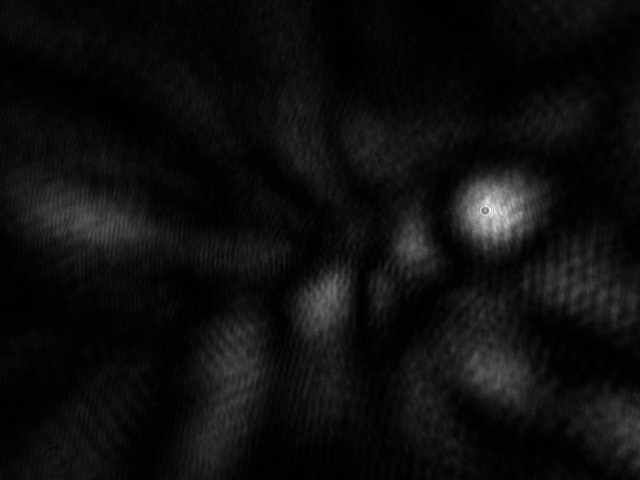
\includegraphics[width=\textwidth]{PicA1000}
    \caption{}
  \end{subfigure}
  \begin{subfigure}[b]{0.5\textwidth}
    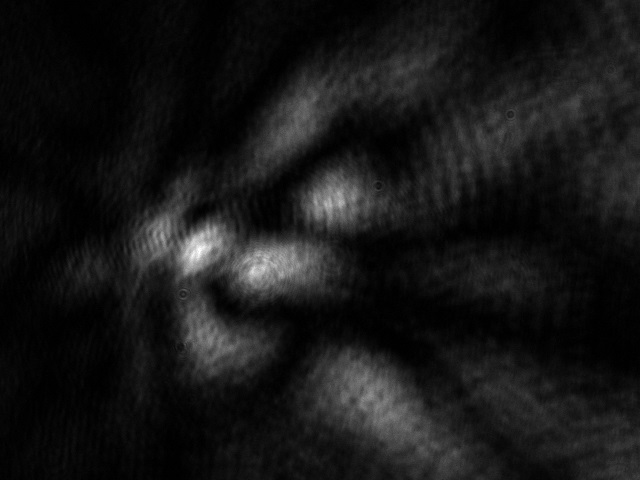
\includegraphics[width=\textwidth]{PicA1001}
    \caption{}
  \end{subfigure}
  \begin{subfigure}[b]{0.5\textwidth}
    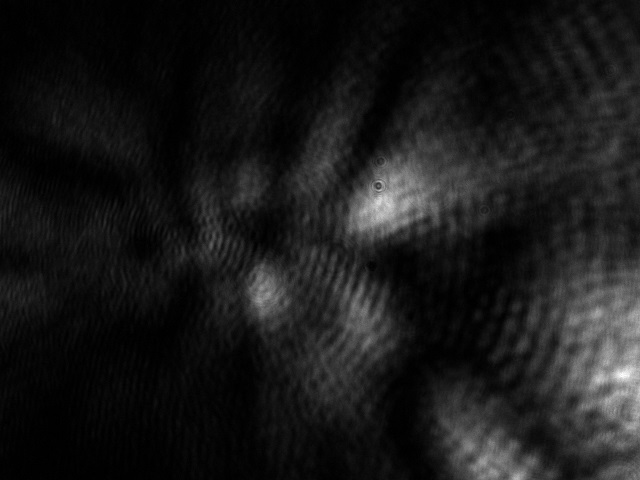
\includegraphics[width=\textwidth]{PicA1002}
    \caption{}
  \end{subfigure}
  \begin{subfigure}[b]{0.5\textwidth}
    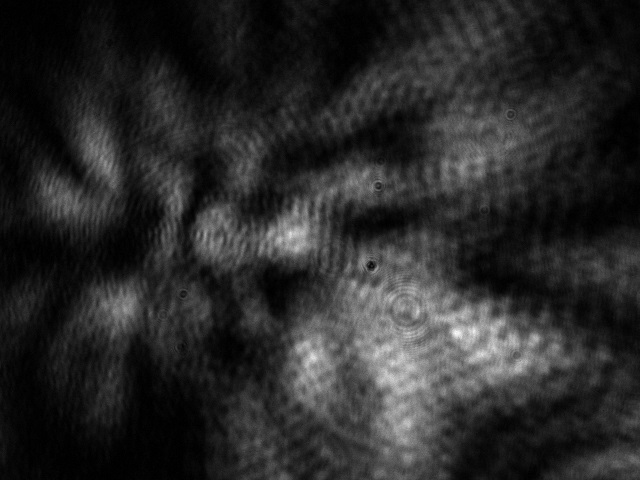
\includegraphics[width=\textwidth]{PicA1003}
    \caption{}
  \end{subfigure}
  \caption{The test input for verifying GLCM applications}
\end{figure}
In Table 2.5, we select five textural features from a total 17 features to compare. Based on the comparison of results from MATLAB and C++, we can assume that either one of the codes has or both of them have bugs or defects so that the requirements are not satisfied well. To prove that, another application was implemented in JAVA, which is discussed in the previous section. 
\begin{table}[!b]
\begin{center}
\begin{tabular}{||c c c ||}
& Image (a) & \\
\hline
Feature & MATLAB & C++ \\[0.7ex]
\hline\hline
COR & 0.985299 & 0.984588 \\
DIS & 2.20703 & 2.234017 \\
CON & 10.06387 & 10.63786 \\
IDM & 0.380147 & 0.407319 \\
ASM & 0.005497 & 0.013697 \\
\hline
\end{tabular}
\vspace{0.5cm}
\begin{tabular}{||c c c ||}
& Image (b) & \\
\hline
Feature & MATLAB & C++ \\[0.7ex]
\hline\hline
COR & 0.990801 & 0.990473 \\
DIS & 2.459202 & 2.487369 \\
CON & 12.97538 & 13.50661 \\
IDM & 0.364664 & 0.387451 \\
ASM & 0.003817 & 0.009142 \\
\hline
\end{tabular}
\begin{tabular}{||c c c ||}
& Image (c) & \\
\hline
Feature & MATLAB & C++ \\[0.7ex]
\hline\hline
COR & 0.991887 & 0.991633 \\
DIS & 2.626308 & 2.651188 \\
CON & 14.99225 & 15.53600 \\
IDM & 0.355747 & 0.380085 \\
ASM & 0.003739 & 0.009151 \\
\hline
\end{tabular}
\begin{tabular}{||c c c ||}
& Image (d) & \\
\hline
Feature & MATLAB & C++ \\[0.7ex]
\hline\hline
COR & 0.989492 & 0.989358 \\
DIS & 3.956470 & 3.969021 \\
CON & 30.91669 & 31.39502 \\
IDM & 0.254904 & 0.272799 \\
ASM & 0.001061 & 0.002534 \\
\hline
\end{tabular}
\caption {The feature values calculated from MATLAB and C++ for images in Figure 2.4}
\end{center}
\end{table}
At the beginning, the JAVA code is only implemented for calculating the COR, DIS, CON, IDM and ASM texture feature parameters for verification purposes. By using the same four diffraction images shown in Figure 2.4 as test inputs, we unfortunately got another version of results that is different from the MATLAB and C++ ones. In Table 2.6, we present the comparison of results for Figure 2.4(a). 
\begin{table}[!t]
\begin{center}
\begin{tabular}{||c c c c||}
\hline
Feature & MATLAB & C++ & JAVA\\[0.7ex]
\hline\hline
COR & 0.985299 & 0.984588 & 0.962522 \\
DIS & 2.20703 & 2.234017 & 6.818101\\
CON & 10.06387 & 10.63786 & 82.14295 \\
IDM & 0.380147 & 0.407319 & 0.217207 \\
ASM & 0.005497 & 0.013697 & 0.005483\\
\hline
\end{tabular}
\caption{The texture feature results of Figure 2.4(a)}
\end{center}
\end{table}
From these results, we can't prove the assumption until we verify that the JAVA application meets the requirements. We apply the JUnit testing for major components comprising loadImage, calculationGLCM and GLCMFeatures. Consequently, we construct an 10-by-10 array of pixels ranging from 0 to 9 
\begin{align*}
I = 
\renewcommand{\arraystretch}{0.5}
\begin{bmatrix}
    1 & 6 & 2 & 3 & 9 & 3 & 0 & 6 & 2 & 8\\
    6 & 5 & 4 & 4 & 8 & 6 & 5 & 3 & 3 & 8\\
    0 & 9 & 7 & 0 & 0 & 6 & 8 & 2 & 6 & 7\\
    1 & 6 & 7 & 9 & 7 & 5 & 6 & 4 & 2 & 2\\
    5 & 7 & 1 & 2 & 2 & 6 & 2 & 4 & 7 & 5\\
    1 & 4 & 4 & 1 & 4 & 6 & 3 & 1 & 9 & 0\\
    7 & 4 & 5 & 3 & 5 & 2 & 4 & 5 & 7 & 4\\
    7 & 7 & 4 & 2 & 8 & 1 & 9 & 2 & 3 & 3\\
    7 & 1 & 6 & 4 & 4 & 9 & 1 & 3 & 5 & 1\\
    1 & 1 & 6 & 3 & 9 & 2 & 8 & 5 & 1 & 2
\end{bmatrix}
\end{align*}
as a test input to represent an image. By manually creating GLCM along the $0^0$ direction from the array of pixels, we achieve the GLCM
\begin{align*}
G_0 = 
\renewcommand{\arraystretch}{0.5}
\begin{bmatrix}
    1&     0&     0&     0&     0&     0&      2&     0&     0&     1\\
    0&     1&     2&     1&     2&     0&     4&     0&     0&     2\\
    0&     0&     2&     2&     2&     0&     2&     0&     3  &   0\\
    1&     1&     0&     2&     0&     2&     0&     0&     1 &    2\\
    0&     1&     2&     0&     3&     2&     1&     1 &    1  &   1\\
    0 &    2  &   1  &   2   &  1  &   0  &   1 &    2&     0  &   0\\
    0&     0&     3&     2&     2&     2&     0&     2&     1  &   0\\
    1&     2&     0&     0&     3&     2&     0&     1 &    0  &   1\\
    0 &    1  &   1   &  0   &  0  &   1 &    1&     0&     0  &   0\\
    1&     1&     2&     1&     0&     0&     0&     2&     0  &   0
\end{bmatrix}
\end{align*}
Based on the GLCM, we calculate the values of texture feature parameters COR, DIS, CON, IDM and ASM which are the expected outputs. Therefore, we create a test case including the test input I and expected output G for the JAVA application that is treated as execution condition. Through the verification process, we achieve the result shown in Table 2.7. 
\begin{table}[!h]
\begin{center}
\begin{tabular}{|| c | c  c | c ||}
\hline
Texture Feature & expected Result & Actual Result & Passed \\
\hline\hline
COR & 0.999965 & 0.999965 & Y \\
DIS & 290.0 & 290.0 & Y \\
CON & 1432.0 & 1432.0 & Y \\
IDM & 22.749199 & 22.749199 & Y\\
ASM & 174.0 & 174.0 & Y\\
\hline
\end{tabular}
\end{center}
\caption{Testing result for JAVA application}
\end{table}
As the table shows, all actual results are matched with expected results, which indicates the JAVA application can satisfy the requirements and achieve the correct feature values. To cover all possible GLCMs created along all directions, we perform the same process for $45^0$, $90^0$ and $135^0$ angles and manually create the GLCM for the remaining single direction:
\begin{align*}
G_{45} = 
\renewcommand{\arraystretch}{0.5}
\begin{bmatrix}
     0&     0&     0&     0&     0 &    1&     1&     0&     1&     0\\
     0&     2&     2&     0&     2 &    0&     1&     2&     0&     2\\
     0&     1&     0&     2&     1 &    2&     0&     3&     0&     0\\
     0&     0&     1&     1&     4 &    0&     0&     0&     1&     0\\
     0&     3&     2&     2&     1 &    0&     2&     0&     1&     1\\
     0&     1&     1&     1&     0 &    1&     3&     0&     1&     1\\
     1&     0&     3&     0&     1 &    1&     2&     1&     1&     0\\
     2&     0&     1&     0&     3 &    1&     1&     2&     0&     0\\
     0&     0&     1&     3&     0 &    0&     0&     0&     0&     0\\
     1&     0&     0&     0&     1 &    2&     0&     0&     0&     2
\end{bmatrix}
G_{90} = 
\begin{bmatrix}
     0&     0&     0&     0&     1&     1&     1&     0&     1&     0\\
     1&     1&     2&     1&     1&     2&     0&     3&     0&     1\\
     0&     1&     0&     2&     0&     1&     3&     2&     0&     2\\
     0&     1&     3&     0&     2&     0&     1&     1&     0&     0\\
     1&     1&     4&     2&     2&     1&     0&     1&     1&     0\\
     1&     2&     1&     2&     2&     0&     2&     0&     0&     0\\
     0&     1&     0&     2&     1&     1&     3&     0&     1&     1\\
     1&     1&     1&     0&     2&     0&     1&     3&     1&     1\\
     0&     1&     0&     0&     0&     2&     0&     0&     1&     1\\
     1&     1&     0&     0&     2&     1&     0&     1&     0&     0
\end{bmatrix}
\end{align*}
\begin{align*}
G_{135} = 
\renewcommand{\arraystretch}{0.5}
\begin{bmatrix}
     0&     0&     0&     0 &    2 &    0 &    0 &    1  &   0  &   0\\
     0&     2&     1&     2 &    0 &    1 &    1 &    2  &   0  &   0\\
     0&     0&     1&     0 &    3 &    4 &    1 &    1  &   0  &   1\\
     1&     0&     0&     0 &    1 &    1 &    3 &    1  &   0  &   1\\
     0&     1&     3&     0 &    2 &    1 &    3 &    1  &   1  &   1\\
     1&     3&     2&     2 &    1 &    0 &    0 &    0  &   0  &   0\\
     1&     1&     1&     1 &    0 &    0 &    1 &    2  &   1  &   1\\
     1&     2&     0&     1 &    1 &    1 &    0 &    1  &   0  &   1\\
     0&     0&     1&     2 &    0 &    0 &    1 &    0  &   0  &   1\\
     0&     0&     1&     0 &    2 &    0 &    1 &    1  &   1  &   0
\end{bmatrix}
\end{align*}
Based on these GLCMs, we further create the average GLCM from all directions by dividing the sum for each element in the GLCM by 4. The average GLCM is 
\begin{align*}
G_{ave} = 
\renewcommand{\arraystretch}{0.5}
\begin{bmatrix}
0.25 &0 &0 &0 &0.75 &0.5 &1 &0.25 &0.5 &0.25\\
0.25 &1.5 &1.75 &1 &1.25 &0.75 &1.5 &1.75 &0 &1.25\\
0 &0.5 &0.75 &1.5 &1.5 &1.75 &1.5 &1.5 &0.75 &0.75\\
0.5 &0.5 &1 &0.75 &1.75 &0.75 &1 &0.5 &0.5 &0.75\\
0.25 &1.5 &2.75 &1 &2 &1 &1.5 &0.75 &1 &0.75\\
0.5 &2 &1.25 &1.75 &1 &0.25 &1.5 &0.5 &0.25 &0.25\\
0.5 &0.5 &1.75 &1.25 &1 &1 &1.5 &1.25 &1 &0.5\\
1.25 &1.25 &0.5 &0.25 &2.25 &1 &0.5 &1.75 &0.25 &0.75\\
0 &0.5 &0.75 &1.25 &0 &0.75 &0.5 &0 &0.25 &0.5\\
0.75 &0.5 &0.75 &0.25 &1.25 &0.75 &0.25 &1 &0.25 &0.5
\end{bmatrix}
\end{align*}
Through operating the calculationGLCM method, all GLCMs generated from the JAVA application are the same as the expected results. 
Although we confirm that the texture features can be correctly calculated from GLCM, as well as that the GLCM can be created from the array of pixels, we must verify whether the array of pixels can represent the image correctly or not. Because of the complexity of image data, it is impossible to manually create the expected output for an image. Instead, we considered using a verified method to generate the expected output from images such as the imread() method in MATLAB. However, when we compare some elements with the same position in the matrix, the values are different. We pick 27-pixel values of images ranging from 10 to 255 in the matrix generated from the imread() method and choose the same number of the pixel value in the same position of a matrix created from the JAVA application. By building a map between each pixel value from MATLAB and its corresponding value from JAVA, we can obviously see the nonlinear trend shown in Figure 2.5, 
\begin{figure}[!h]
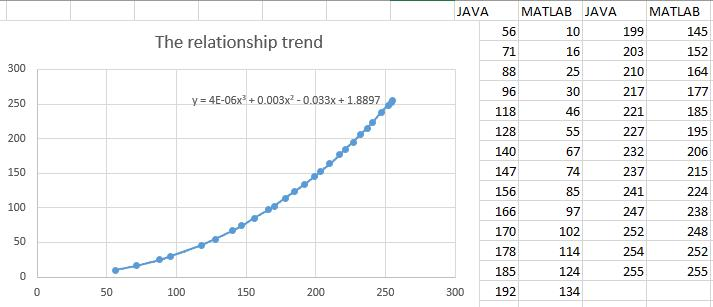
\includegraphics[width = \linewidth]{rgb_statistical}
\caption{The nonlinear relationship between JAVA and MATLAB result}
\end{figure}
which means we failed to create the correct pixel matrix from the image using the JAVA application. Through some research, we discovered that the misuse of the class Color is the reason of getting the wrong matrix. Instead of the class Color, the class Raster is the correct choice for a Gray-level image. The problem is caused by default color space sRGB, a proposed standard RGB color space, in Color class. Also, in BufferedImage class, the method getRGB() returns an integer pixel in default color model TYPE\_INT\_ARGB, while the color model of our images is TYPE\_BYTE\_GRAY. Thus, we replace the Color class with the Raster class. After fixing the defects existing in loadingImage class, we use the Figure 2.4(a) as input to run the JAVA application again and receive the new result shown in Table 2.8. 
\begin{table}[!t]
\begin{center}
\begin{tabular}{||c c c c||}
\hline
Feature & MATLAB & C++ & JAVA\\[0.7ex]
\hline\hline
COR & 0.985299 & 0.984588 & 0.985184 \\
DIS & 2.207030 & 2.234017 & 2.232489\\
CON & 10.06387 & 10.63786 & 10.13244 \\
IDM & 0.380147 & 0.407319 & 0.375932 \\
ASM & 0.005497 & 0.013697 & 0.005439\\
\hline
\end{tabular}
\caption{The texture feature results of Figure 2.4(a) after modification}
\end{center}
\end{table}
From the result, we can see there are still three different versions of feature results, but for the JAVA application, all components have passed the verification process, and all possible directions for creating GLCM are covered within the testing procedure. Thus, we can confirm the assumption that both the C++ application and MATLAB script contain defects, and the JAVA application can be applied in the future research.\par
To further research the reason for the difference between the MATLAB tool and the newly developed JAVA application, we compare the GLCM created from each tool. Given the test input image in Figure 2.4(a), the MATLAB script generates the GLCM which is the same as the GLCM created by the JAVA application. Due to the result, we can verify that the MATLAB script can create the correct GLCM. Additionally, in MATLAB, there is a built-in method to create the GLCM. Thus, the difference in texture feature values comes from the algorithms of texture feature calculations. By perform static testing for the MATLAB script, we find the primary reason that causes the difference is the time of normalizing the GLCM. The MATLAB script normalizes the GLCM after the average GLCM is achieved, while the JAVA application normalizes the GLCM after GLCM along with each direction is created. To conclude, there are no functional defects in the MATLAB script. However, we apply the JAVA application in processing diffraction images because it provides simple UI for users so that we can modify the parameters of GLCM without changing the specific code.  

\section{Diffraction Images Pre-Classification and Feature Calculation}
In this experiment, we are provided 6000 diffraction images within which there are 3000 diffraction image pairs. Each image pair contains two diffraction images captured at the same time by two cameras with s-polarizer or p-polarizer placed separately in front of them. All diffraction images we use in the experiment are 8-bit color, so the gray levels of an image are 256 ranging from 0 to 255. In addition, the resolution of these images is 640x480. Thus, the array of pixels is a 640-by-480 matrix with the maximum number of each element as 255. For identification purposes, the diffraction image pair has the same name before the symbol (-) and different numbers (1 or 2) after the symbol. For instance, the 2015040718412300745-1.bmp means the p-polarized image, whereas the 2015040718412300745-2.bmp means the s-polarized image. There is some research using the similar approach to acquiring diffraction images, such as the classification of Jurkat T and Ramos B cells\cite{Feng} and the analysis of cellular objects through diffraction images\cite{Zhang}. \par
The primary goal of this research is to validate whether or not the SVM algorithm can be applied for image classification based on texture features. In general, SVM is a supervised learning algorithm in machine learning. The training data set should be classified first. For all diffraction images in this research, we label them with three different categories based on the pattern recognition of diffraction image. These three types are cell, debris, and strip. Some image pairs for each group are shown in Figures 2.6, 2.7 and 2.8. 
\begin{figure}[!h]
\centering
  \begin{subfigure}[b]{0.2\textwidth}
    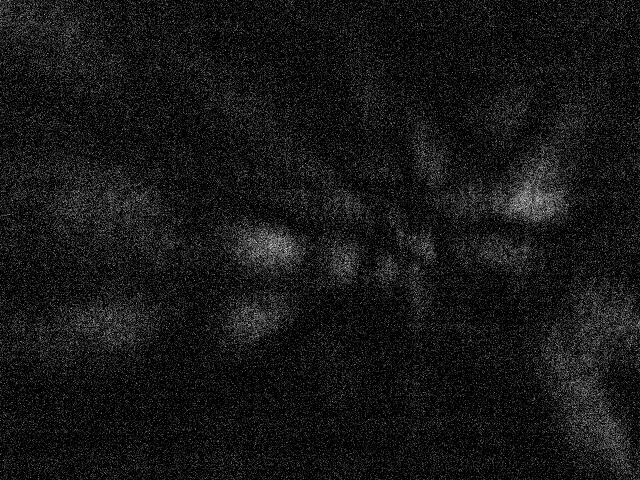
\includegraphics[width=\textwidth]{diffraction_image/2015040117594700171-1}
    \caption{p-polarized}
  \end{subfigure}
  \begin{subfigure}[b]{0.2\textwidth}
    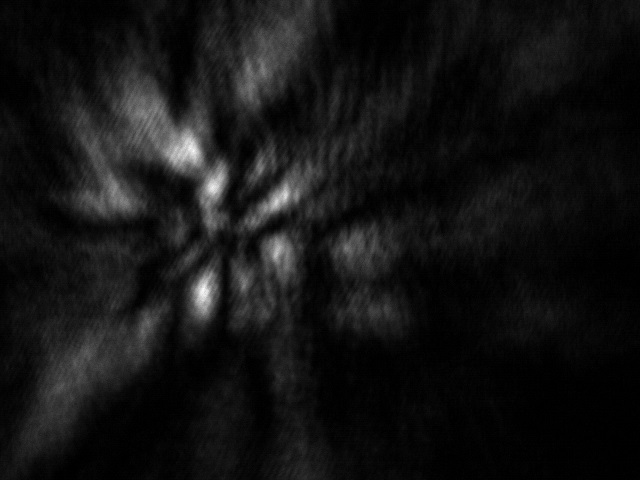
\includegraphics[width=\textwidth]{diffraction_image/2015040117594700171-2}
    \caption{s-polarized}
  \end{subfigure}
  \begin{subfigure}[b]{0.2\textwidth}
    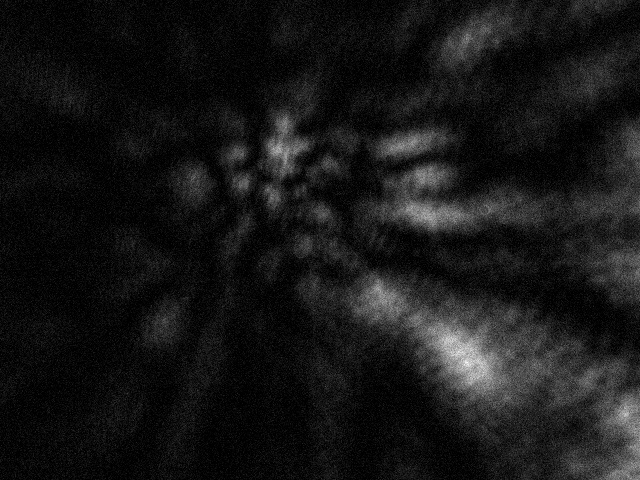
\includegraphics[width=\textwidth]{diffraction_image/2015040117594700185-1}
    \caption{p-polarized}
  \end{subfigure}
  \begin{subfigure}[b]{0.2\textwidth}
    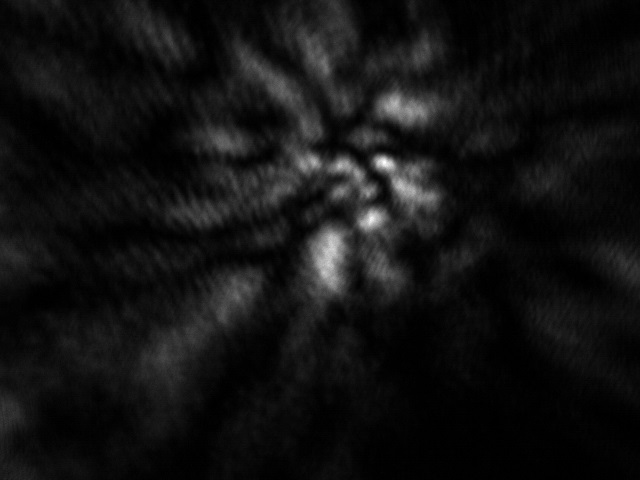
\includegraphics[width=\textwidth]{diffraction_image/2015040117594700185-2}
    \caption{s-polarized}
  \end{subfigure}
  \caption{Diffraction images classified as Cell type}
\end{figure}
\begin{figure}[!h]
\centering
  \begin{subfigure}[b]{0.2\textwidth}
    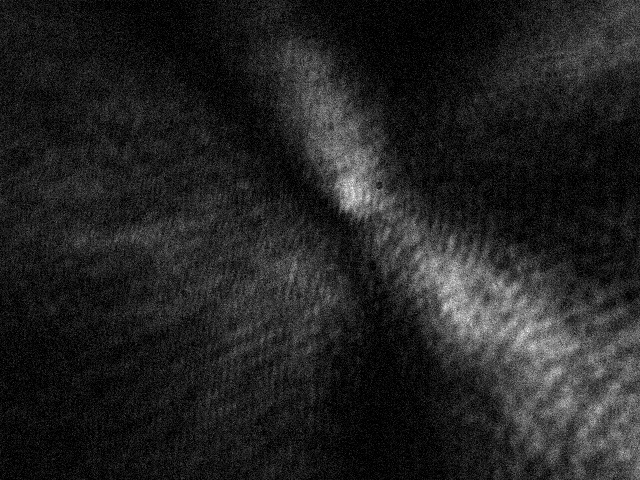
\includegraphics[width=\textwidth]{diffraction_image/2015040117594700004-1}
    \caption{p-polarized}
  \end{subfigure}
  \begin{subfigure}[b]{0.2\textwidth}
    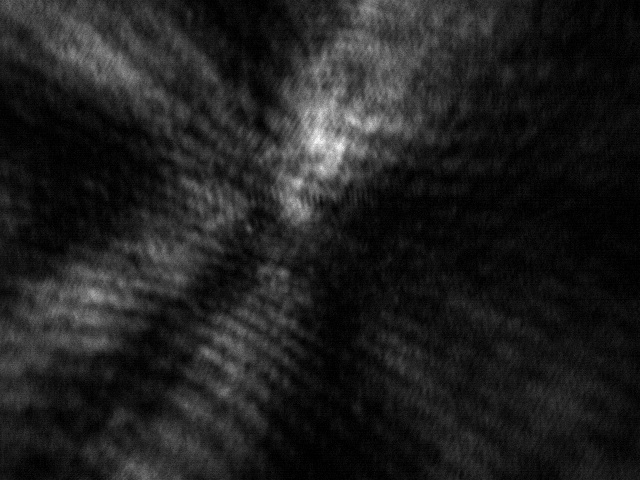
\includegraphics[width=\textwidth]{diffraction_image/2015040117594700004-2}
    \caption{s-polarized}
  \end{subfigure}
  \begin{subfigure}[b]{0.2\textwidth}
    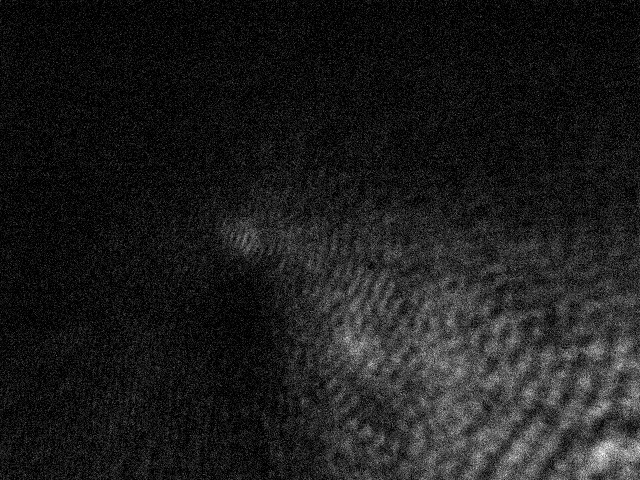
\includegraphics[width=\textwidth]{diffraction_image/2015040117594700050-1}
    \caption{p-polarized}
  \end{subfigure}
  \begin{subfigure}[b]{0.2\textwidth}
    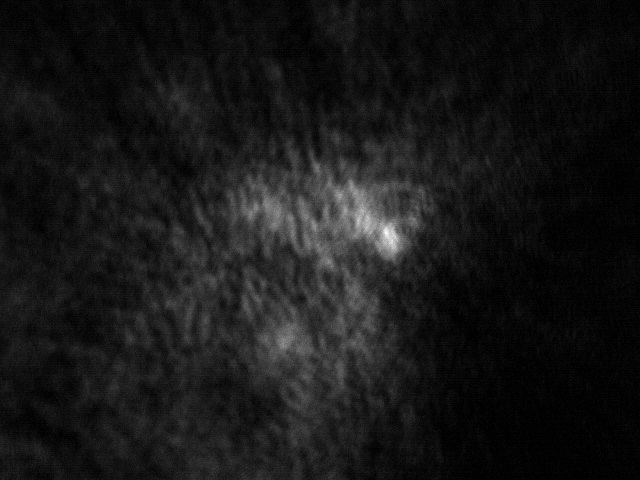
\includegraphics[width=\textwidth]{diffraction_image/2015040117594700050-2}
    \caption{s-polarized}
  \end{subfigure}
  \caption{Diffraction images classified as Debris type}
\end{figure}
\begin{figure}[!h]
\centering
  \begin{subfigure}[b]{0.2\textwidth}
    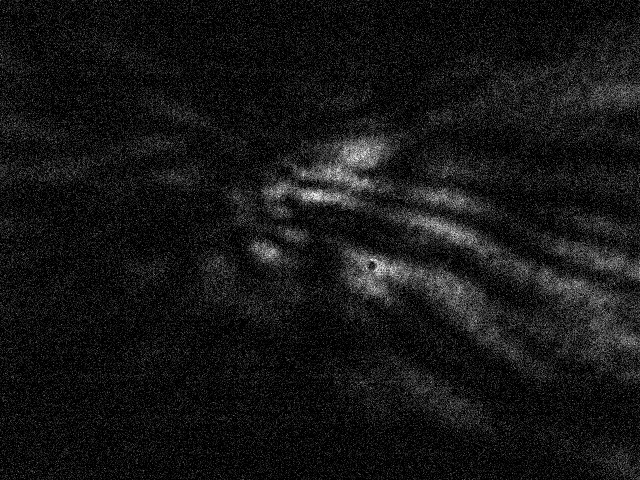
\includegraphics[width=\textwidth]{diffraction_image/2015040117594700071-1}
    \caption{p-polarized}
  \end{subfigure}
  \begin{subfigure}[b]{0.2\textwidth}
    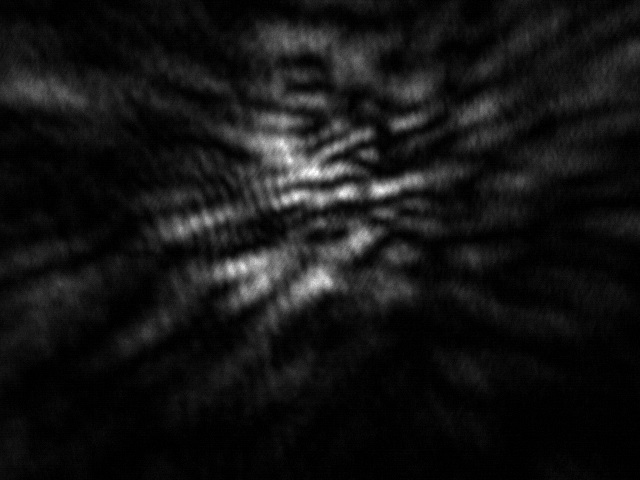
\includegraphics[width=\textwidth]{diffraction_image/2015040117594700071-2}
    \caption{s-polarized}
  \end{subfigure}
  \begin{subfigure}[b]{0.2\textwidth}
    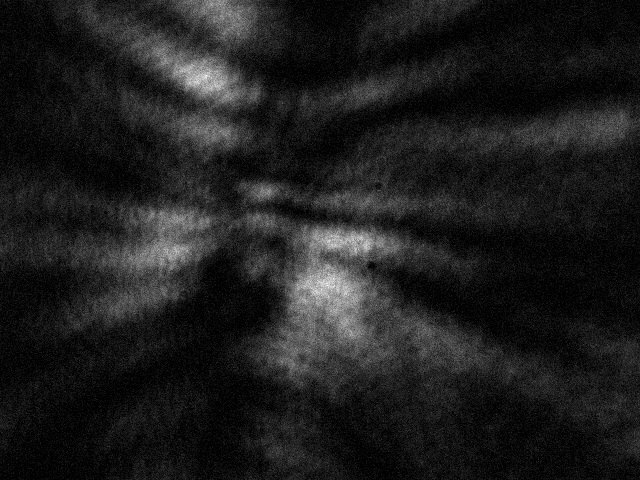
\includegraphics[width=\textwidth]{diffraction_image/2015040117594700158-1}
    \caption{p-polarized}
  \end{subfigure}
  \begin{subfigure}[b]{0.2\textwidth}
    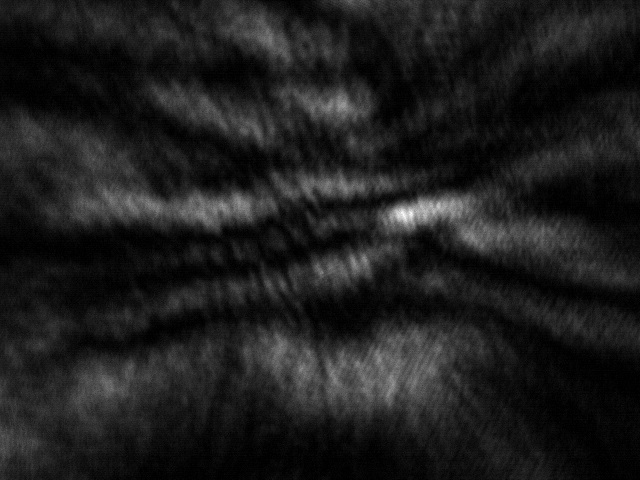
\includegraphics[width=\textwidth]{diffraction_image/2015040117594700158-2}
    \caption{s-polarized}
  \end{subfigure}
  \caption{Diffraction images classified as Strip type}
\end{figure}
Because of the complexity of the pattern recognition of diffraction image, the accuracy cannot be guaranteed. Through the pre-classification process, we have 957 image pairs in the cell folder, 1555 image pairs in the debris folder, and 488 pairs in the strip folder. To process this image data, we operate the JAVA application and set up the offset and angular direction parameters shown in Figure 2.9. 
\begin{figure}
\centering
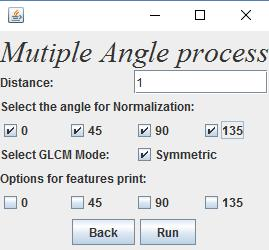
\includegraphics{java_panel}
\caption{JAVA application main panel}
\end{figure}
As it shows, the distance between two pixels is 1 and the application processes the diffraction image data along with all directions. Because of having the symmetry checked, each value of an element in GLCM along with each direction is doubled. In the meantime, the value of each element in GLCM is divided by the number of created GLCMs, as well as normalized by the total amount of occurrences of valid reference pixel values. Eventually, the application generates three CSV files, Cell.CSV, Debris.csv, and Strip.csv, as the results that are used in the automated classification research later. 
\section{Conclusion}
In this section, we focus on image texture analysis. The pattern recognition of diffraction image is complex because its representation is abstract. In this research, we try to use two diffraction images captured at the same time but from different directions to improve its representation and the performance of its pattern recognition. GLCM is a statistical method for texture feature analysis. We develop an application in JAVA to verify and supplement two existing tools. The newly developed application provides a simple UI so that users can modify GLCM parameters without changing the code. We perform system testing for three tools and unit testing for the JAVA application. The result of system testing reveals that the two existing tools have trouble in satisfying the requirements. The unit testing for loading image components reveals the bug that leads the JAVA application to convert the diffraction image data into an incorrect pixel matrix. Through debugging this component, we replace the class Color in JAVA library with the class Raster. We also perform static testing between the MATLAB and JAVA tools. The difference in texture feature values is caused by the time of performing the normalization process for GLCM. All image data used in this research are pre-classified into three types of diffraction image: cell, debris, and strip. The pre-classification process is based on the experience of people, so the accuracy cannot be guaranteed. Finally, we process all image data through the JAVA application. We receive 3000 data examples of which there are 957 examples labeled as cell type, 1555 examples labeled as debris type, and 488 examples labeled as strip type.  Further classification will be performed by SVM using texture features extracted in this section. In the meantime, we will validate whether the texture features can be applied in SVM for classification. 